\definecolor{c82b366}{RGB}{130,179,102}
\definecolor{cd5e8d4}{RGB}{213,232,212}
\definecolor{c9673a6}{RGB}{150,115,166}
\definecolor{ce1d5e7}{RGB}{225,213,231}
\definecolor{c6c8ebf}{RGB}{108,142,191}
\definecolor{cdae8fc}{RGB}{218,232,252}
\definecolor{c666666}{RGB}{102,102,102}
\definecolor{whitesmoke}{RGB}{245,245,245}


\def \globalscale {0.850000}
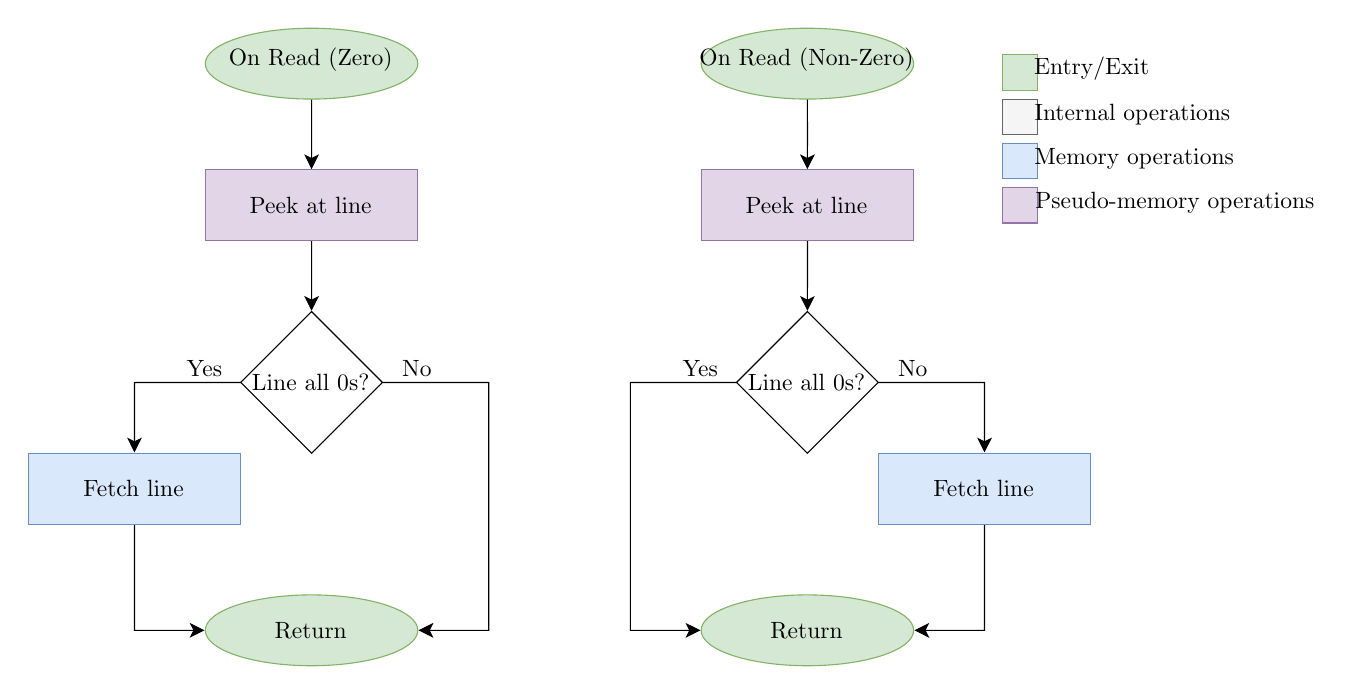
\begin{tikzpicture}[y=1cm, x=1cm, yscale=\globalscale,xscale=\globalscale, every node/.append style={scale=\globalscale}, inner sep=0pt, outer sep=0pt]
  \path[draw=black,miter limit=10.0] (4.2333, 8.4931) -- (4.2341, 7.9632) -- (4.2336, 7.6033);



  \path[draw=black,fill=black,miter limit=10.0] (4.2333, 7.4644) -- (4.141, 7.6496) -- (4.2336, 7.6033) -- (4.3262, 7.6494) -- cycle;



  \path[draw=c82b366,fill=cd5e8d4] (4.2333, 9.0223) ellipse (1.5875cm and 0.5292cm);



  \begin{scope}[fill=black,anchor=south]
    \node[text=black,anchor=south] (text1268) at (4.2201, 8.9032){On Read (Zero)};



  \end{scope}
  \path[draw=black,miter limit=10.0] (4.2341, 6.3765) -- (4.2341, 5.8465) -- (4.2336, 5.4867);



  \path[draw=black,fill=black,miter limit=10.0] (4.2333, 5.3478) -- (4.141, 5.533) -- (4.2336, 5.4867) -- (4.3262, 5.5327) -- cycle;



  \path[draw=c9673a6,fill=ce1d5e7] (2.6458, 7.4348) rectangle (5.8208, 6.3765);



  \begin{scope}[fill=black,anchor=south]
    \node[text=black,anchor=south] (text4814) at (4.2201, 6.7866){Peek at line};



  \end{scope}
  \path[draw=black,miter limit=10.0] (1.5883, 2.1431) -- (1.5883, 0.5548) -- (2.4773, 0.5556);



  \path[draw=black,fill=black,miter limit=10.0] (2.6162, 0.5556) -- (2.431, 0.4628) -- (2.4773, 0.5556) -- (2.431, 0.648) -- cycle;



  \path[draw=c6c8ebf,fill=cdae8fc] (0.0, 3.2015) rectangle (3.175, 2.1431);



  \begin{scope}[fill=black,anchor=south]
    \node[text=black,anchor=south] (text3543) at (1.5743, 2.5532){Fetch line};



  \end{scope}
  \path[draw=c82b366,fill=cd5e8d4] (4.2333, 0.5556) ellipse (1.5875cm and 0.5292cm);



  \begin{scope}[fill=black,anchor=south]
    \node[text=black,anchor=south] (text3650) at (4.2201, 0.4366){Return};



  \end{scope}
  \path[draw=black,miter limit=10.0] (3.1758, 4.259) -- (1.5883, 4.259) -- (1.5875, 3.37);



  \path[draw=black,fill=black,miter limit=10.0] (1.5875, 3.2311) -- (1.4952, 3.4163) -- (1.5875, 3.37) -- (1.6804, 3.4163) -- cycle;



  \path[draw=black,miter limit=10.0] (5.2909, 4.259) -- (6.88, 4.259) -- (6.88, 0.5548) -- (5.9894, 0.5556);



  \path[draw=black,fill=black,miter limit=10.0] (5.8505, 0.5556) -- (6.0357, 0.648) -- (5.9894, 0.5556) -- (6.0357, 0.4628) -- cycle;



  \path[draw=black,fill=white,miter limit=10.0] (4.2333, 5.3181) -- (5.2917, 4.2598) -- (4.2333, 3.2015) -- (3.175, 4.2598) -- cycle;



  \begin{scope}[fill=black,anchor=south]
    \node[text=black,anchor=south] (text1381) at (4.2201, 4.1407){Line all 0s?};



  \end{scope}
  \path (2.1167, 4.8683) rectangle (3.175, 4.0746);



  \begin{scope}[fill=black,anchor=south]
    \node[text=black,anchor=south] (text6353) at (2.6326, 4.3524){Yes};



  \end{scope}
  \path (5.2917, 4.8683) rectangle (6.35, 4.0746);



  \begin{scope}[fill=black,anchor=south]
    \node[text=black,anchor=south] (text8222) at (5.8076, 4.3524){No};



  \end{scope}
  \path[draw=black,miter limit=10.0] (11.6417, 8.4931) -- (11.6425, 7.9632) -- (11.6419, 7.6033);



  \path[draw=black,fill=black,miter limit=10.0] (11.6417, 7.4644) -- (11.5493, 7.6496) -- (11.6419, 7.6033) -- (11.7345, 7.6494) -- cycle;



  \path[draw=c82b366,fill=cd5e8d4] (11.6417, 9.0223) ellipse (1.5875cm and 0.5292cm);



  \begin{scope}[fill=black,anchor=south]
    \node[text=black,anchor=south] (text2645) at (11.6284, 8.9032){On Read (Non-Zero)};



  \end{scope}
  \path[draw=black,miter limit=10.0] (11.6425, 6.3765) -- (11.6425, 5.8465) -- (11.6419, 5.4867);



  \path[draw=black,fill=black,miter limit=10.0] (11.6417, 5.3478) -- (11.5493, 5.533) -- (11.6419, 5.4867) -- (11.7345, 5.5327) -- cycle;



  \path[draw=c9673a6,fill=ce1d5e7] (10.0542, 7.4348) rectangle (13.2292, 6.3765);



  \begin{scope}[fill=black,anchor=south]
    \node[text=black,anchor=south] (text6142) at (11.6284, 6.7866){Peek at line};



  \end{scope}
  \path[draw=black,miter limit=10.0] (14.2883, 2.1431) -- (14.2883, 0.5548) -- (13.3977, 0.5556);



  \path[draw=black,fill=black,miter limit=10.0] (13.2588, 0.5556) -- (13.444, 0.648) -- (13.3977, 0.5556) -- (13.444, 0.4628) -- cycle;



  \path[draw=c6c8ebf,fill=cdae8fc] (12.7, 3.2015) rectangle (15.875, 2.1431);



  \begin{scope}[fill=black,anchor=south]
    \node[text=black,anchor=south] (text3619) at (14.2743, 2.5532){Fetch line};



  \end{scope}
  \path[draw=c82b366,fill=cd5e8d4] (11.6417, 0.5556) ellipse (1.5875cm and 0.5292cm);



  \begin{scope}[fill=black,anchor=south]
    \node[text=black,anchor=south] (text4780) at (11.6284, 0.4366){Return};



  \end{scope}
  \path[draw=black,miter limit=10.0] (12.6992, 4.259) -- (14.2883, 4.259) -- (14.2875, 3.37);



  \path[draw=black,fill=black,miter limit=10.0] (14.2875, 3.2311) -- (14.1952, 3.4163) -- (14.2875, 3.37) -- (14.3804, 3.4163) -- cycle;



  \path[draw=black,miter limit=10.0] (10.5841, 4.259) -- (8.9966, 4.259) -- (8.9966, 0.5548) -- (9.8856, 0.5556);



  \path[draw=black,fill=black,miter limit=10.0] (10.0245, 0.5556) -- (9.8393, 0.4628) -- (9.8856, 0.5556) -- (9.8393, 0.648) -- cycle;



  \path[draw=black,fill=white,miter limit=10.0] (11.6417, 5.3181) -- (12.7, 4.2598) -- (11.6417, 3.2015) -- (10.5833, 4.2598) -- cycle;



  \begin{scope}[fill=black,anchor=south]
    \node[text=black,anchor=south] (text3655) at (11.6284, 4.1407){Line all 0s?};



  \end{scope}
  \path (12.7, 4.8683) rectangle (13.7583, 4.0746);



  \begin{scope}[fill=black,anchor=south]
    \node[text=black,anchor=south] (text6546) at (13.2159, 4.3524){No};



  \end{scope}
  \path (9.525, 4.8683) rectangle (10.5833, 4.0746);



  \begin{scope}[fill=black,anchor=south]
    \node[text=black,anchor=south] (text7304) at (10.0409, 4.3524){Yes};



  \end{scope}
  \path[draw=c82b366,fill=cd5e8d4] (14.5521, 9.1546) rectangle (15.0813, 8.6254);



  \path (14.9754, 9.2869) rectangle (16.8275, 8.4931);



  \begin{scope}[fill=black,anchor=south]
    \node[text=black,anchor=south] (text3001) at (15.8882, 8.7709){Entry/Exit};



  \end{scope}
  \path[draw=c666666,fill=whitesmoke] (14.5521, 8.4931) rectangle (15.0813, 7.964);



  \path (14.9225, 8.6254) rectangle (18.0975, 7.8317);



  \begin{scope}[fill=black,anchor=south]
    \node[text=black,anchor=south] (text3021) at (16.4968, 8.1095){Internal operations};



  \end{scope}
  \path[draw=c6c8ebf,fill=cdae8fc] (14.5521, 7.8317) rectangle (15.0813, 7.3025);



  \path (14.8167, 7.964) rectangle (18.2563, 7.1702);



  \begin{scope}[fill=black,anchor=south]
    \node[text=black,anchor=south] (text3178) at (16.5232, 7.448){Memory operations};



  \end{scope}
  \path[draw=c9673a6,fill=ce1d5e7] (14.5521, 7.1702) rectangle (15.0813, 6.641);



  \path (14.896, 7.3025) rectangle (19.394, 6.5088);



  \begin{scope}[fill=black,anchor=south]
    \node[text=black,anchor=south] (text4354) at (17.1318, 6.7866){Pseudo-memory operations};



  \end{scope}

\end{tikzpicture}
